\documentclass[12pt,a4paper,Spanish]{article}
%Va a ser un libro (book), el tamaño es a4, la lengua castellano%%%

%\[spanish]{babel} %palabras de multitud de idiomas. Aquí no se si 
\usepackage[utf8]{inputenc} %cambio latin por utf-8
\usepackage{amsmath} %macros AM
\usepackage{amsthm} %macros AMS para teoremas.
\usepackage{amsfonts} %Permite usar fuentes.
%\usepackage[dvips]{epsfig} %Inclusión de figuras postscript
\usepackage{indentfirst}
\usepackage{graphicx}
\usepackage{subfigure}
\usepackage{afterpage}
\usepackage{float}
\newcommand\blankpage{%
	\null
	\thispagestyle{empty}%
	\newpage}
\usepackage{hyperref}
\usepackage{afterpage}
\setlength{\parskip}{8mm} %Separación entre parrafos 
\usepackage{multirow, array} % para las tablas
%\usepackage{longtable} % para tablas largas
\usepackage[left=3 cm,top=2.5cm,right=3cm,bottom=2.5cm]{geometry} 
%\usepackage{cite} % para contraer referencias
\usepackage[utf8]{inputenc}
\usepackage[backend=biber]{biblatex}
\addbibresource{biblio.bib}
\usepackage{setspace}
\usepackage{titlesec}
\spacing{1.5}
\DeclareGraphicsExtensions{.jpg, .pdf, .png, .gif, .eps}
% para nivel 4 de secciones
\setcounter{secnumdepth}{4} 
\setcounter{tocdepth}{4}
\titleformat{\paragraph}
{\normalfont\normalsize\bfseries}{\theparagraph}{1em}{}
\titlespacing*{\paragraph}
{0pt}{3.25ex plus 1ex minus .2ex}{1.5ex plus .2ex}



\begin{document}

\renewcommand{\listtablename}{Índice de tablas} 

%% --------------- PORTADA -----------------------%%

\begin{titlepage}
\begin{center}
\begin{figure}
	\centering

\includegraphics[width=0.3\textwidth]{./figs/logoURJC}
\end{figure}
\begin{center}
\large
ESCUELA DE INGENIERÍA DE FUENLABRADA
\vspace*{0.15in}
GRADO EN INGENIERÍA DE SISTEMAS AUDIOVISUALES Y MULTIMEDIA \\
\vspace*{0.6in}
{\large \bf TRABAJO FIN DE GRADO}\\
\end{center}
\vspace*{0.2in}
{\large
{TÍTULO} \\
}
\vspace*{0.3in}
\vspace*{0.3in}
\vspace*{0.1in}
\end{center}
{\large
Autor: Víctor Iglesias Cuevas  \\[0.2cm]
Tutora: Rebeca Goya Esteban \\[0.15cm]
}
\vspace*{0.1in}
\vspace*{0.1in}
\begin{center}Curso académico 2023/2024\end{center}
\end{titlepage}


%% ------------------- CITA --------------------- %%
\newpage
\thispagestyle{empty} % para que no se numere esta pagina
%\pagenumbering{Roman} % para comenzar la numeracion de paginas en numeros romanos
\begin{flushright}
	\vspace*{5cm}
 	\textit{“esto es una cita" (el que hizo la cita)}
\end{flushright}





%% ------------------- AGRADECIMIENTOS --------------------- %%
\newpage
\thispagestyle{plain}
\section*{Agradecimientos} % si no queremos que añada la palabra "Capitulo"
\addcontentsline{toc}{section}{Agradecimientos} % si queremos que aparezca en el índice
%\markboth{AGRADECIMIENTOS}{AGRADECIMIENTOS} % encabezado 

aquí van los agradecimientos









%% -------------------- RESUMEN --------------------%%
\newpage
\section*{Resumen}
\addcontentsline{toc}{section}{Resumen} % si queremos que aparezca en e
Esto es un resumen











%%%%%%%%%%%%%% - INDICE - %%%%%%%%%%%%%
\newpage
\renewcommand*\contentsname{ÍNDICE} % Se modifica el nombre por defecto de la "Table Of Contents" (tabla de contenidos, índice) para pasar a llamarla "ÍNDICE".
\tableofcontents
\afterpage{\blankpage} % Se añade una página en blanco después del índice.




%%%%%%%%%%%%%% - INDICE DE TABLAS- %%%%%%%%%%%%%
\newpage
\renewcommand{\listtablename}{ÍNDICE DE TABLAS} % Se define el nombre del índice de tablas.
\listoftables % Se genera automáticamente el índice con las distintas tablas del documento (entorno \table o \longtable).
\addcontentsline{toc}{section}{ÍNDICE DE TABLAS} % Se añade manualmente el apartado al índice (Table Of Contents, TOC).




%%%%%%%%%%%%%% - INDICE DE FIGURAS- %%%%%%%%%%%%%
\newpage
\renewcommand{\listfigurename}{ÍNDICE DE FIGURAS} % Se define el nombre del índice de figuras.
\listoffigures % Se genera automáticamente el índice con las distintas figuras del documento (entorno \figure).
\addcontentsline{toc}{section}{ÍNDICE DE FIGURAS} % Se añade manualmente el apartado al índice (Table Of Contents, TOC).






%%%%%%%%%%%%%% - INTRODUCCIÓN- %%%%%%%%%%%%%
\newpage
%\pagenumbering{arabic} % para empezar la numeración con números
\section{Introducción}
\subsection{Motivación y contexto}
La música juega un rol importante en la vida de la personas, aun más en la era digital. El uso de Internet ha contribuido enormemente en el crecimiento de librerías digitales de música, y con ello, la información y metadatos disponibles de cada pista de audio. El poder emocional de la música es el motivo de su aplicación en áreas tan diversas como la industria del juego, la industria cinematográfica, marketing y musicoterapia, pero los conocimientos científicos sobre este fenómeno están lejos de ser completos o reveladores \cite{eerola2012review}.
\newline
La relación entre música y emoción ha sido objeto de muchos debates académicos e investigaciones empíricas en muchas disciplinas diferentes donde están incluidas la filosofía, la musicología, la psicología, la biología, la antropología y la sociología. Sin embargo, no fue hasta la década de los 2000, cuando el estudio de este tema desde el punto de vista de la ingeniería, comenzó a desarrollar un modelo computacional de emoción musical para la recuperación y organización de la música basada en emociones \cite{yang2011music}.
\newline
Tradicionalmente, la clasificación de música ha estado basada en catálogos de metadatos (artista, album, título de la canción, ...) \cite{yang2011music}. Esta clasificación puede no ser suficiente para el usuario. Tener acceso a una categorización de la música en función de emociones o estados de ánimo puede ser de gran utilidad para muchas aplicaciones. Imaginemos un reproductor de música que, además de recomendarte canciones según un grupo o un estilo musical, sea capaz de hacerlo según el estado de ánimo que tengas.
\newline
Aquí es donde entra en juego el Reconocimiento Musical de Emociones (Music Emotion Recognition). MER categoriza emociones y aplica técnicas de Machine Learning (Aprendizaje Máquina) para clasificarlas usando diferentes características extraídas de la señal acústica de la canción \cite{yang2011music}.
\newline
En este trabajo blablablablabla..........

\subsection{Objetivos del trabajo}
El objetivo principal del trabajo es diseñar un sistema para el reconocimiento de emociones en pistas de audio.
Los objetivos específicos que se plantean son los siguientes:
\begin{itemize}
\item Estudiar el Estado del Arte de los sistemas MER
\item Examinar técnicas de Aprendizaje Máquina (Machine Learning) para la detección de emociones
\item Usar lenguage Python para:
 	\begin{itemize}
 		\item procesar de datos del banco de datos 
 		\item desarrollar algoritmos de Machine Learning
 		\item entrenar y probar los sistemas para ajustar parámetros
 		\item evaluar las técnicas de Machine Learning según su capacidad para predecir los valores requeridos 		
 	\end{itemize}
\end{itemize}

\subsection{Metodología y estructura de la memoria}
La memoria está compuesta por cuatro apartados:
\begin{enumerate}
	\item Una introducción de la memoria donde se expone el contexto y la motivación del trabajo.
	\item El capítulo de \textit{Estado del arte} donde se expone:
	\begin{itemize}
		\item una introducción a la campo de estudio MER,
		\item una descripción de Machine Larning y los diferentes tipos de algoritmos que hay, 
		\item y una explicación de los modelos de regresión y algunos de los ejemplo más comunes
	\end{itemize}
	\item El capítulo de \textit{Experimentos} dividido en:
	\begin{itemize}
		\item descripción de los datos utilizados,
		\item y los algoritmos de Machine Learning empleados en el trabajo
	\end{itemize}
	\item Los resultados detallados de los experimentos realizados en el capítulo anterior.
	\item Las conclusiones obtenidas del trabajo, y líneas futuras en las que seguir profundizando en MER.
\end{enumerate}









%%%%%%%%%%%%%% - ESTADO DEL ARTE - %%%%%%%%%%%%%
\newpage
\section{Estado del arte}
\subsection{Music Emotion Recognition}

Music Emotion Recognition (MER) es un campo de estudio que se enfoca en identificar y clasificar las emociones que la música evoca en los oyentes. Para ello, se extraen las características relevantes de las pistas de audio, se procesan, se evalúan, y posteriormente se asocian con determinadas emociones \cite{GomezCanon2021SPM}.
\newline
MER es una de las disciplinas de alto nivel más desafiantes en Music Information Retrieval (MIR). MIR un campo de investigación que se centra en la extracción e inferencia de características significativas de la música (a partir de la señal de audio), la clasificación de la música utilizando estas características, y el desarrollo de diferentes esquemas de búsqueda y recuperación. Tiene como objetivo poner a disposición de los individuos el vasto almacén de música del mundo \cite{schedl2014music}

\subsubsection{Emociones}\label{emo}

Los modelos teóricos de la emoción adoptados por los estudios se dividieron en cuatro clases: discretos, dimensionales, misceláneos y específicos de la música \cite{eerola2012review}. 
\newline
Uno de los más comunes usado en psicología es el modelo dimensional propuesto por Russell \cite{posner2005circumplex}. El modelo consiste en la representación de las emociones a través de dos dimensiones: valencia ( nivel de agrado o desagrado) y excitación (representa el nivel de energia o activación de la valencia). Cada emoción es una representación linea de la combinación de estas dos dimensiones

\begin{figure}[H]
	\centering
	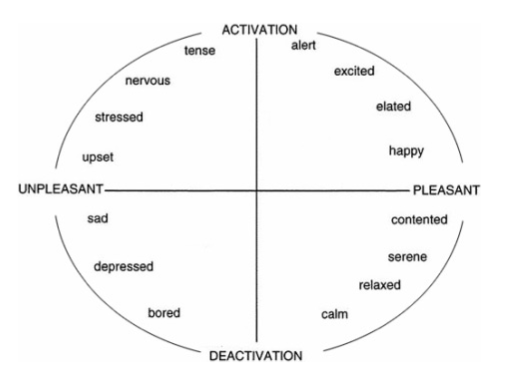
\includegraphics[width=0.7\linewidth]{figs/russell}
	\caption{Modelo dimensional de Russell}
	\label{fig:russell}
\end{figure}


Un aspecto importante en MER es la categorización de las emociones según su naturaleza. Se distinguen dos tipos:
\begin{itemize}
\item Percibidas: son aquellas que hacen referencia a las características musicales canción: tono, escala, ritmo, etc.
\item Inducidas: son las emociones que hacen referencia al contexto individual de cada persona
\end{itemize}
\cite{yang2011music} expone un ejemplo claro para distinguir entre los dos tipos: el Cumpleaños Feliz. Si analizamos la canción por sus características, se podría decir que es una canción alegre (emoción percibida). Pero es posible que para algunas personas les produzca tristeza al asociar un recuerdo con esta canción (emoción inducida)

\subsubsection{Estado actual MER}
El flujo de trabajo se divide en cuatro bloques \cite{GomezCanon2021SPM}:


\paragraph{Taxonomía y propiedades musicales de la emoción}\label{tax_emo}
Es la forma en que se clasifican y categorizan las emociones. Hay dos taxonomías predominantes en el marco actual de MER:
\begin{itemize}
	\item Enfoque categórico/discreto presenta diferentes clases: feliz, triste, etc. Este enfoque tiene una resolución mala y resulta ambiguo
	\item Enfoque dimensional. Como explica el apartado anterior, se conceptualiza la emoción como un elemento bidimensional (valencia y excitación). Este enfoque puede resultar más exacto que el anterior, pero también más complejo a la hora de mapear las emociones en el marco que propone Russell \cite{posner2005circumplex}
\end{itemize}
La elección de la taxonomía es la decisión más importante para diseñar un conjunto de datos, y define el nivel de precisión emocional.

\paragraph{Creación del conjunto de datos y recopilación de anotaciones subjetivas}
La forma más utilizada para la recopilación de emociones musicales es la subjetiva. Los anotadores suelen escuchar extractos de canciones (de unos 30 segundos) para posteriormente emitir juicios emocionales. Los datos son anotados siguiendo la taxonomía elegida para la creación del conjunto de datos. Estos anotadores son expertos en música, pero sin conocimiento alguno de teoría musical (musicólogos, productores, investigadores, etc.).
\newline
Todas las calificaciones son promediadas para llegar a una "verdad universal". Es decir, los valores finales son un promedio de las anotaciones de cada experto.

\paragraph{Extracción de las características}
En los conjuntos de datos se encuentran características de dos tipos: propiedades acústicas a bajo nivel y los niveles musicales a alto nivel. Estos dos tipos de características no tienen por qué estar relacionadas: las propiedades acústicas a bajo nivel se obtienen de la señal acústica de la canción, mientras que los niveles musicales a alto nivel están relacionados con la melodía, ritmo o el tono.
\newline
A esta diferencia de características se la denomina "brecha semántica". La tendencia actual está enfocada en trabajar para reducir esta brecha: se ha descubierto que el ritmo está relacionado con la estructura métrica y la duración de las notas, o que la dinámica de la canción está relacionada con el volumen, la energía media cuadrática o la intensidad de las notas.


Las herramientas más utilizadas para la extracción de características son:
\begin{itemize}
	\item MIRToolbox. Un conjunto de herramientas en Matlab.
	\item OpenSMILE. Desarrollada en C++.
	\item Essentia 4. Desarrollado en C++, posee clasificadores previamente entrenados.
	\item PsySound. Librería para uso en Matlab basada en algoritmos psicoacústicos
	\item Librosa. Biblioteca de código abierto para Python. Especializada en el análisis y procesamiento de audio y música. Es ampliamente utilizada en la comunidad de investigación en musicología, así como en aplicaciones prácticas que involucran el procesamiento y análisis de señales de audio en MIR.
\end{itemize}

\paragraph{Evaluación}
La evaluación de los sistemas MER está directamente relacionada con la taxonomía de las emociones: la taxonomía elegida para trabajar en el sistema MER afecta a las características extraídas y los valores a predecir, y estos a su vez a la evaluación de los sistemas. Hay dos enfoques de sistema MER:
\begin{itemize}
	\item Sistema de clasificación si la taxonomía elegida sigue un enfoque categórico/discreto. Los parámetros de evaluación de estos sistemas son los mismos que en modelos de clasificación de otras disciplinas: precisión, f-score, precision, etc.
	\item Sistema de regresión si el enfoque es dimensional/continuo. Los parámetros comúnmente usados para evaluar estos sistemas son: error cuadrático medio, coeficiente de determinación (R2) o coeficiente de correlación de Pearson ($\rho$).
\end{itemize}





\begin{figure}[H]
	\centering
	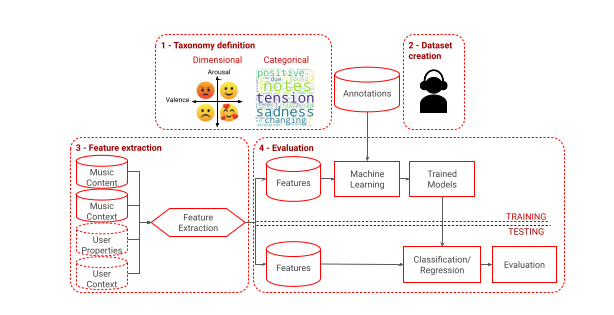
\includegraphics[width=0.7\linewidth]{figs/mer_traditional_system}
	\caption{Sistema tradicional MER}
	\label{fig:mertraditionalsystem}
\end{figure}


\subsubsection{Estado futuro MER}
En el libro \citetitle{yang2011music} se presentan varias vías de trabajo donde MER puede profundizar:

\paragraph{Timbre vocal}
Actualmente, en el análisis emocional de una canción, MER pone el foco en la música y en las letras. Sin embargo, la voz contiene muchos matices que pueden resultar  especialmente valiosos en los modelos de predicción. Los timbres de voz (alegre, rasgado, agudo, agresivo, etc.) afectan a la percepción que tiene el oyente de la canción.
\newline
Existen distintas formas de estudiar el timbre vocal basadas en el estudio de la señal acústica de la voz y la extracción de descriptores (pitch, energía, coficientes cepstrum, ...).

\paragraph{Factores de situación}
En el apartado ~\ref{emo} donde se describen las emociones, se hace referencia a las emociones inducidas. La situación del oyente (momento del día, si está acompañado o solo, etc) afecta directamente a las emociones inducidas. El estudio de la situación puede ser de ayuda para dar contexto acerca del entorno que tiene el oyente, y modificar (o no) la predicción de emociones.

\paragraph{Conexión entre enfoques dimensional y categórico}
Como se describe en el apartado ~\ref{tax_emo} hay dos enfoques bien diferenciados en el estudio de MER: dimensional/continuo y categórico/discreto. una combinación de los dos enfoques puede resultar eficaz

\subsection{Técnicas de Aprendizaje Máquina}

El aprendizaje máquina (Machine Learning) es la ciencia de programar ordenadores para que estos puedan aprender de los datos \cite{geron2022hands}. Se enfoca en la idea de que los ordenadores puedan "aprender" a partir de la experiencia y los datos: identifican patrones en los datos y predicen o deciden en función de esos patrones. La idea es partir del sistema de etiquetado de emociones (enfoque categórico) y encontrar su lugar en el espacio valencia-activación que propone el enfoque dimensional. Esto ayudaría a la creación de conjuntos de datos desde el punto de vista del oyente: es más fácil identificar una emoción que situarla dentro del espacio valencia-activación 

\subsubsection{Tipos de Machine Learning}
Los tipos de Machine Learning se clasifican en diferentes categorías según su naturaleza \cite{geron2022hands}:
\begin{itemize}
	\item Grado de supervisión humana durante el entrenamiento. Dentro de esta categoría se encuentran los siguientes sistemas:
	\begin{itemize}
		\item supervisados,
		\item no supervisados,
		\item refuerzo del aprendizaje (Reinforcement Learning)
	\end{itemize}
	\item Si pueden o no aprender de forma incremental. se distinguen dos tipos:
	\begin{itemize}
		\item sistemas en línea (Batch Learning),
		\item sistemas por lotes (Online Learning)
	\end{itemize}
	\item Si detectan o no patrones en los datos de entrenamiento, construyendo un modelo predictivo. Tipos:
	\begin{itemize}
		\item basados en instancias,
		\item basados en modelos
	\end{itemize}
\end{itemize}
Estos criterios no son exclusivos. Pueden combinarse de la forma que se quiera.

\subsubsection{Sistemas supervisados vs. no supervisados}
Los sistemas supervisados de Machine Learning son algoritmos que utilizan datos etiquetados (etiquetas) durante la fase de entrenamiento del sistema. Son utilizados tanto para modelos de clasificación como para modelos de regresión (predicción de un número dado un paquete de características). Algunos de los algoritmos supervisados más importantes son:
\begin{itemize}
	\item KNN vecinos
	\item Regresión lineal
	\item Regresión logarítmica
	\item Redes Neuronales	
\end{itemize}
Por otro lado nos encontramos los sistemas no supervisados. Se utilizan para encontrar patrones o estructuras ocultas en datos. A diferencia de los supervisados, estos algoritmos no utilizan ningún etiquetado ni requieren de ninguna salida deseada durante el entrenamiento. Tipos de algoritmos no supervisados:
\begin{itemize}
	\item Agrupamiento (Clustering)
	\begin{itemize}
		\item K-medias
		\item DBSCAN
		\item Análisis de agrupamiento jerárquico (HCA)	
	\end{itemize}
	\item Detección de anomalías
	\begin{itemize}
		\item One-class SVM
		\item Isolation Forest	
	\end{itemize}
	\item Reducción de visualización
	\begin{itemize}
		\item Análisis de componentes principales (PCA)
		\item Kernel PCA	
		\item Locally-Linear Embedding (LLE)
		\item t-distributed Stochastic Neighbor Embedding (t-SNE)
	\end{itemize}
	\item Aprendizaje de reglas de asociación
	\begin{itemize}
		\item Apriori
		\item Eclat	
	\end{itemize}	
\end{itemize}

\subsubsection{Batch Learning y Online Learning}
Los sistemas Batch Learning son incapaces de aprender de forma incremental. El modelo se entrena utilizando la totalidad del conjunto de datos de entrenamiento de una sola vez, en lugar de hacerlo de manera incremental o en pequeñas partes. Dada la forma de entrenar, estos sistemas son capaces de captar mejor las complejidades y las variabilidades de los datos. Sin embargo, son más vulnerables frente a cambios en los datos puesto que sería necesario volver a entrenar el modelo de nuevo.
\newline
Los sistemas Online Learning son lo contrario a los anteriores: se entrenan de forma incremental. Se dividen los datos en pequeñas instancias (o mini-batches) y se alimenta el sistema de forma secuencial. Cada aprendizaje es rápido y barato. Se utiliza para sistemas donde se reciben datos de forma continua, o cuando se requiere una gran cantidad de datos para el entrenamiento. En estos modelos es importante el parámetro de tasa de aprendizaje (learning rate): Una tasa de aprendizaje alto hará que el sistema se adapte bien a cambios en los datos, pero también será más susceptible a olvidar más rápido datos antiguos


\subsubsection{Basados en instancias y Basados en modelos}
Esta clasificación hace referencia a cómo los sistemas de aprendizaje se generalizan. Por un lado están los basados en instancias: el sistema aprende los ejemplos de memoria y luego generaliza a nuevos casos comparándolos con los ejemplos aprendidos (o un subconjunto de
ellos). Es decir, utiliza una medida de similitud. Estos sistemas tiene un buen rendimiento con datos entrenados, pero no es suficiente para un sistema de Machine Learning: el verdadero objetivo es tener un buen rendimiento en instancias nuevas.
\newline
Aquí es donde se encuentran los sistemas basados en modelos, cuya forma de generalizar es a partir de modelos que hagan predicciones. Estos sistemas tienen mucho mejor rendimiento frente a instancias de datos muy ruidosas (gran cantidad de datos aleatorios). Para conseguir buenos resultados con estos sistemas se deben seguir algunos pasos como: selección del modelo (elegir el mejor modelo que se adapte a nuestro sistema), ajuste del modelo (elección correcta de los parámetro o hiperparámetros),  o entrenamiento el modelo.

\subsection{Modelos de Regresión}
Los modelos de Regresión son técnicas que se utilizan para predecir un valor numérico continuo basado en una o más variables independientes. Para ello, se modela el efecto de un conjunto de variables explicativas sobre una varibale de interés primario \autocite{fahrmeir2013regression}.
\newline
Los conceptos fundamentales de los modelos de Regresión son:
\begin{itemize}
	\item Variable Dependiente (variable objetivo, respuesta o de interés primario): es la variable que se desea predecir. Esta puede ser continua, binaria, categórica o de recuentos
	\item Variables explicativas: también llamadas covariables, variables independientes o regresoras. Son las que se utiliza para predecir la variable dependiente. Existen varios tipos de estas variables como continuas, binarias,	o categóricas. En modelos complejos también es posible incluir escalas temporales, variables para describir la distribución espacial o la ubicación geográfica, o indicadores grupales.
	\item Tipo de modelo: dependerá principalmente del tipo de variable respuesta, y del tipo de variables independientes
\end{itemize}
Una característica principal de los modelos de regresión es que la relación entre la variable independiente y las variables independientes no es una función determinista, si no que muestra errores. Esto implica que la respuesta \textit{y} es una variable aleatoria, cuya distribución depende de las variables independientes. Un ejemplo claro sería: sabiendo la altura de los padres no se puede predecir exactamente la altura de los hijos, solo estimar una media y el grado de dispersión. A esta desviación del valor esperado se la denomina $\epsilon$ (componente aleatorio o estocástico) (por eso es muy importante estudiar la importancia de las covariables en el valor medio de la variable objetivo). La función resultante es un modelo condicional donde los valores de \textit{y} (variable objetivo) están condicionados por las covariables ($x_1, x_2, x3, ...$) y el componente aleatorio $\epsilon$:

\begin{equation}
	y = E(y|x_1, ..., x_k) = f(x_1, ..., x_k) + \epsilon 
\end{equation}


\subsubsection{Árboles de decisión}\label{decision_tree}
Los árboles de decisión son una técnica de Machine Learning y estadística utilizada tanto para casos de clasificación como para casos regresión. Son modelos predictivos que representan decisiones y sus posibles consecuencias, incluidas las probabilidades de diferentes resultados. Son conceptualmente simples, pero poderosos
\newline
El principio de los árboles de regresión es segmentar el espacio características en una serie de regiones simples. El conjunto de reglas de división utilizadas para segmentar el espacio se pueden resumir en un árbol, de ahí el término \cite{gareth2013introduction}.
\newline
En el libro \citetitle{hastie2009elements} se explican los modelos de decisión con un ejemplo simple: imaginemos un problema de regresión con una respuesta continua $Y$ y los inputs $X_1$ y $X_2$. Primero se divide el espacio en dos regiones. Se elige la variable y el punto de divisón para lograr el mejor ajuste. Luego, una o ambas regiones se dividen en dos regiones más. Continúa el proceso hasta que se aplica alguna regla de detención.



\subsubsection{Bosques aleatorios}
Los árboles aleatorios (random forests) son un método de aprendizaje para clasificación y regresión que consiste en construir una multitud de árboles de decisión (ver ~\ref{decision_tree}) en la etapa de entrenamiento, y así obtener el modo de las clases (clasificación) o la media de las predicciones (regresión) de los árboles individuales.
\newline
La idea de los bosques aleatorios es reducir la varianza del sistema, reduciendo la correlación entre los árboles (sin incrementar en exceso la varianza). Esto es posible gracias a una selección aleatoria de variables independientes durante el proceso de crecimiento de los árboles \cite{hastie2009elements}.
\newline
La forma en que se construye los bosques aleatorios es la siguiente:
\begin{enumerate}
	\item Se elige el número $B$ de árboles de decisión que formará el bosque
	\item Se hace crecer los árboles del bosque repitiendo de forma recursiva los siguientes pasos
	\begin{enumerate}
		\item Del conjunto de datos de entrenamiento, se elige un subconjunto aleatorio de las características (generalmente $\sqrt{\rho}$ variables si hay $\rho$ en total).
		\item De este subconjunto, se elige la mejor variable .
		\item Se dividen los nodos en dos nodos hijos.
	\end{enumerate}
	\item Se obtienen los datos del conjunto de árboles.
	\item Se hace la predicción.
\end{enumerate}


\subsubsection{Regresión Lineal}
La regresión lineal es uno de los métodos más básicos y  utilizados de regresión. Aquí tienes una definición más detallada. Como se explica en el apartado anterior, en regresión existe una relación entre la variable objetivo y las variables independientes a través de la función $f(x1, ..., xk)$. Esta función no es exacta al estar afectada por el ruido $\epsilon$. El objetivo es estimar función desconocida $f$, es decir, separar el componente sistemático de $f$ del ruido aleatorio $\epsilon$, asumiendo en este caso un acercamiento lineal \cite{fahrmeir2013regression}. La ecuación resultante es la siguiente:
\begin{equation}
	y_i = 
	\beta_0 + \beta_1x_i, ..., \beta_kx_i + \epsilon_i = 
	 x'_i\beta + \epsilon 
\end{equation}
 
Donde los parámetros $\beta_0, \beta_1, ..., \beta_k$ son desconocidos y deben ser estimados. El parámetro $\beta_0$ respresenta la intersección (cuando el valor de $x$ es 0).
\newline
\begin{figure}[H]
	\centering
	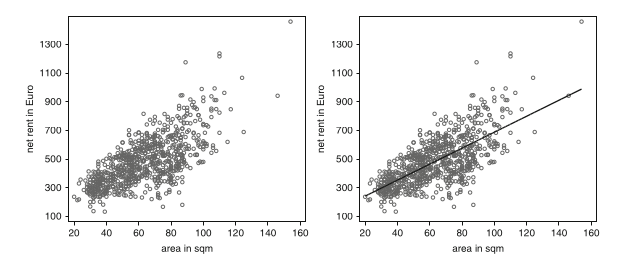
\includegraphics[width=0.7\linewidth]{figs/linear_regression}
	\caption{Regresión Lineal}
	\label{fig:linearregression}
\end{figure}
El objetivo de la regresión lineal es encontrar la mejor línea recta que minimiza la suma de los errores cuadrados (diferencias entre los valores reales y los valores predichos).

\subsubsection{Ridge}
La regresión ridge es una variante de la regresión lineal estándar. Modifica la estimación de los coeficientes del modelo para mejorar la precisión: introduce una penalización que reduce los coeficientes de las variables independientes. Para lograr esta penalización se agrega un término de regulación que es proporcional a la suma de los cuadrados de los coeficientes. La fórmula de la regresión ridge es la siguiente \cite{hastie2009elements}:
\begin{equation}
	\hat{\beta}^{ridge} = argmin {\sum_{i=1}^{N}} (y_i - \beta_0 - \sum_{j=1}^{p}x_{ij}\beta^{2}_j)
\end{equation}
\newline
Donde:
\begin{itemize}
	\item $\hat{\beta}^{ridge}$ es el término de regularización ridge
	\item $y_i$ es la variable respuesta para la observación $i$
	\item $x_{ij}$ es el valor de la variable independiente $j$ para la observación $i$
	\item $\beta_{j}$ son los coeficientes del modelo
\end{itemize}

La regresión ridge se utiliza cuando hay muchas variables independientes y se quiere mejorar la precisión del modelo lineal: los coeficientes puede estar mal determinados y mostrar una varianza muy alta. Al imponer una restricción de tamaño de los coeficientes se soluciona este problema \cite{fahrmeir2013regression}.




\begin{figure}[H]
	\centering
	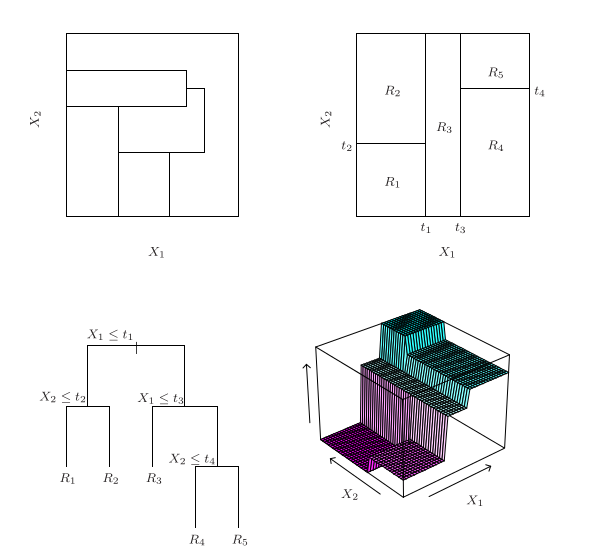
\includegraphics[width=0.7\linewidth]{figs/decission_tree}
	\caption{Funcionamiento de un árbol de decisión}
	\label{fig:decissiontree}
\end{figure}


Los métodos basados en árboles de decisión son simples, y útiles para la interpretación. Sin embargo, normalmente no son competitivos con los mejores enfoques de aprendizaje supervisado en términos de predicción \cite{gareth2013introduction}.







%%%%%%%%%%%%%% - EXPERIMENTOS - %%%%%%%%%%%%%
\newpage
\section{Experimentos}
En este capítulo se describe el proceso del desarrollo de la aplicación MER. Primeramente se describen el conjunto de datos utilizado en el experimento. Seguidamente se describe cómo han sido manipulados los datos para que sean utilizados por el sistema. Por último, se describen las técnicas de Machine Learning utilizadas en la aplicación.


\subsection{Conjunto de datos}
El conjunto de datos elegido para el experimento es DEAM dataset - The MediaEval Database for Emotional Analysis of Music \cite{AlajankiEmoInMusicAnalysis}. El conjunto de datos DEAM consta de 1802 extractos y canciones libres de derechos que provienen de varias fuentes: freemusicarchive.org (FMA), jamendo.com,
y el conjunto de datos medleyDB.
\newline
Existen tres tipos de información claramente diferenciables por cada pista de audio del conjunto de datos: características, valores de valencia y excitación, y metadatos.

\subsubsection{Características}
Los datos presentan un conjunto de características extraídas de la librería openSMILE \cite{openSMILE}. Cada pista de audio está representada en un fichero CSV, donde las pistas se dividen en ventanas de 500ms. En cada ventana se muestran dos valores de cada una de las características: la media y la desviación estándar
Las características presentes en el conjunto de datos son \cite{openSMILEfeatures}:
\begin{itemize}
	\item Energía
	\item Intensidad de fotograma/sonoridad (aproximación)
	\item Espectros de banda crítica (Mel/Bark/Octave, filtros de enmascaramiento triangulares)
	\item Mel-/Bark-Frequency-Cepstral Coefficients (MFCC)
	\item Espectros auditivos
	\item Sonoridad aproximada a partir de espectros auditivos.
	\item Coeficientes perceptivos lineales predictivos (PLP)
	\item Coeficientes cepstrales predictivos lineales perceptivos (PLP-CC)
	\item Coeficientes predictivos lineales (LPC)
	\item Pares espectrales de líneas (LSP, también conocido como LSF)
	\item Frecuencia fundamental (mediante el método ACF/Cepstrum y mediante sumación subarmónica (SHS))
	\item Probabilidad de emisión de voz a partir del pico del espectro ACF y SHS
	\item Calidad de voz: Jitter y Shimmer
	\item Frecuencias de formantes y anchos de banda.
	\item Tasa de cruce por cero y media
	\item Características espectrales (energías de banda arbitrarias, puntos de caída, centroide, entropía, maxpos, minpos, varianza (= dispersión), asimetría, curtosis, pendiente)
	\item Nitidez psicoacústica, armonía espectral.
	\item  CROMA (espectros de semitonos deformados en octavas) y funciones CENS (CROMA suavizado y normalizado de energía)
	\item Funciones derivadas de CHROMA para reconocimiento de acordes y claves
	\item F0 Relaciones de armónicos
\end{itemize}

\subsubsection{Valencia y excitación}
Los datos de valencia y excitación se muestran en el conjunto de datos como valores continuos dentro del rango [1, 9].
\newline
Para la extracción de estos valores, se eligieron 45 segundos de cada canción de forma aleatoria (posteriormente se descartaron los 15 primeros segundos debido a la inestabilidad de las anotaciones al inicio de los clips). Los 45 segundos se dividieron en ventanas de 500ms, y por cada ventana se anotaron 10 valores para de valencia y excitación.
\newline
En el conjunto de datos están presentes todas estas anotaciones, junto con los valores de media y desviación estándar de cada canción. Serán estos últimos lo que se usarán en el desarrollo del trabajo

\subsubsection{Metadatos}
En el conjunto de datos de DEAM \cite{AlajankiEmoInMusicAnalysis} también hay información acerca de las canciones: título de la canción, artista, álbum, géneros musicales y etiquetas

\subsection{Desarrollo}
En este apartado se describen los pasos a seguir en el desarrollo del sistema MER. El sistema está compuesto, en primer lugar, por un procesado de datos: se toman los archivos proporcionados por el conjunto de datos y se manipulan para crear las variables de las que están formados los modelos.
\newline
Para la predicción de emociones, se han elegido los siguientes algoritmos de Machine Learning:
\begin{itemize}
	\item Árbol de decisión
	\item Bosques aleatorios
	\item Regresión lineal
	\item Regresión LASSO
\end{itemize}
En los siguientes apartados se procede a explicar cómo se han diseñado los modelos utilizados para cada uno de los algoritmos.
\newline
La taxonomía de emociones elegida para este experimento es la continua/dimensional (ver apartado ~\ref{tax_emo}). Las emociones están representadas por dos valores: valencia y activación. O visto desde el punto de vista de Machine Learning, hay dos variables objetivo. Para diseñar un sistema MER siguiendo esta taxonomía, es necesario el desarrollo de dos modelos de predicción diferentes para cada algoritmo (uno para valencia y otro para activación).
\newline
Tanto la memoria como el código están disponibles en este repositorio Github \url{https://github.com/viglescue/tfg}. El código fuente de la aplicación MER está dividido en dos archivos: \textit{data-recap.ipynb} con todo el desarrollo correspondiente al procesamiento de datos y archivos del conjunto de datos, y \textit{MER-ML-models.ipynb} con el desarrollo de los diferentes algoritmos para la predicción de emociones. El experimento al completo está desarrollado en lenguaje Python, utilizando cuadernos Jupyter en el entorno de Anaconda. 







\subsubsection{Extracción y manipulación de los datos}
El conjunto de datos de DEAM \cite{AlajankiEmoInMusicAnalysis} organiza los datos de la siguiente forma:
\begin{itemize}
	\item Documentos CSV (uno por cada pista de audio) donde se encuentran los valores de las características de cada canción. En cada documento CSV aparece el valor de cada característica en intervalos de 500ms.
	\item Un archivo CSV con los valores de media y desviación para valencia y activación.
\end{itemize}
La idea es recopilar todos los datos en una tabla para manipularlos mejor. Para ello se ha empleado la librería Pandas \cite{mckinney-proc-scipy-2010} para su uso en lenguage Python.
\newline
Para empezar a construir la tabla, primeramente, se han obtienen los nombres de las características a partir  uno de los archivos CSV que las contienen. Dado que los valores de características están disponibles por intervalos de ms, se ha calculado la media de los valores de cada característica (por cada pista de audio) con el fin de obtener un solo valor por característica y canción. Estos valores serán las variables independientes que se usarán posteriormente en los modelos de ML.
\newline
De otro archivo, se han recopilado los valores de media y activación de cada pista de audio. Estos serán las variables independientes (o variables objetivo) de los modelos.
\newline
El resultado ha sido el documento \textit{recap-data.csv}, el cual contiene todas las variables necesarias para construir los sistemas MER a partir de los diferentes modelos de ML.

\begin{figure}[H]
	\centering
	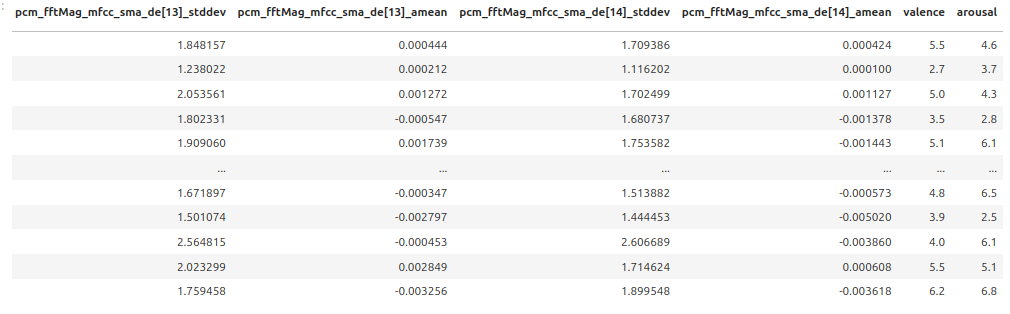
\includegraphics[width=0.7\linewidth]{figs/data}
	\caption{Recopilación de datos}
	\label{fig:data}
\end{figure}



\subsubsection{Regresión Lineal}
\subsubsection{Árbol de regresión}
\subsubsection{RIDGE}
\subsubsection{Bosques aleatorios}




%%%%%%%%%%%%%% - RESULTADOS - %%%%%%%%%%%%%
\newpage
\section{Resultados}







%%%%%%%%%%%%%% - CONCLUSIONES - %%%%%%%%%%%%%
\newpage
\section{Conclusiones}








%%%%%%%%%%%%%% - BIBLIOGRAFÍA - %%%%%%%%%%%%%
\newpage
\section{Bibliografía}
\printbibliography

\end{document}
